\documentclass[11pt]{article}
\usepackage[margin=1in]{geometry}
\usepackage{amsmath,amssymb,amsthm}
\usepackage{graphicx}
\graphicspath{{../figures/}}
\usepackage{xcolor}
\usepackage{booktabs}
\usepackage[numbers,sort&compress]{natbib}
\usepackage[colorlinks=true,linkcolor=blue!50!black,citecolor=blue!50!black,urlcolor=blue!50!black]{hyperref}

\newtheorem{theorem}{Theorem}
\newtheorem{lemma}{Lemma}
\newtheorem{corollary}{Corollary}
\theoremstyle{remark}
\newtheorem{remark}{Remark}

\newcommand{\Hhat}{\hat{H}}
\newcommand{\Vhat}{\hat{V}}
\newcommand{\dd}{\mathrm{d}}
\newcommand{\Ind}[1]{[\,#1\,]}


\title{The instability of negative-mass Schwarzschild\\is a point-mass effect:\\[4pt]
\large Exact thresholds for finite stars}
\author{Nathan Moinvaziri\thanks{\href{mailto:nathan@nathanm.com}{nathan@nathanm.com}}\\[2pt]
\normalsize\textit{Independent researcher}}
\date{October 2026}

\begin{document}
\maketitle

\begin{abstract}
Negative-mass Schwarzschild spacetime is linearly unstable: Gleiser and Dotti exhibited, for every multipole
$\ell\ge2$, an even-parity mode growing as $e^{\gamma t}$ with $\gamma=(\ell-1)\ell(\ell+1)(\ell+2)/(12|M|)$, and
gave numerical evidence that it is the only one. It has been suggested that the instability does not depend on the
singularity and would survive in a regular negative-mass star. We prove, for every $\ell\ge2$, that the
Dotti--Gleiser operator has exactly one negative eigenvalue. The proof uses the zero-energy partner solution
$\phi_0=1/\psi_0$ implicit in their intertwining construction, through a ground-state identity and Glazman's lemma.
The same identity yields an exact count of unstable modes for the exterior of a star of areal radius $R$ whose
interior imposes a Robin condition $\hat\Psi'=\kappa\hat\Psi$:
$\#\{\gamma>0\}=\Ind{R<r_s}+\Ind{\kappa<\kappa_c(R)}$, with $r_s=6|M|/[(\ell+2)(\ell-1)]$ and $\kappa_c$ in closed form.
Consequently the vacuum exterior of any star with $R\ge r_*(\ell)$ ($r_*=2.279|M|$ for $\ell=2$) and a
non-energy-injecting surface condition ($\kappa\ge0$) supports no unstable even-parity mode, and the $\ell^4$ growth
of the point mass is capped by any finite radius. A companion paper applies the count to a regular negative-mass boson star.
\end{abstract}

\section{Introduction}

Bondi's 1957 analysis~\cite{Bondi1957} showed that general relativity contains no logical obstruction to negative
mass, provided inertial, passive and active mass share a sign, and that a pair of equal and opposite masses
self-accelerates (the ``runaway''). Two questions have dominated the subsequent discussion: whether negative mass is
dynamically stable, and whether the runaway is physical. The second was recently addressed by full $3+1$ evolutions of a
canonical boson star paired with a ``phantom'' boson star of negative ADM mass~\cite{Shirokov2026}. Here we address the
first.

For the vacuum point mass the answer is known. Gibbons, Hartnoll and Ishibashi~\cite{GHI2005} proved stability of the
odd-parity sector and, for a range of boundary conditions at the naked singularity, of the even sector. Gleiser and
Dotti~\cite{GD2006} then found exact, smooth, exponentially growing even-parity solutions and showed that the stability
argument of Ref.~\cite{GHI2005} relies on a perturbation that is not continuous at an interior radius where the Zerilli
variable is singular. Dotti and Gleiser~\cite{DG2009} removed that ``kinematic'' singularity with an intertwining
operator, obtained a regular operator $\Hhat$ with a unique self-adjoint extension, and showed that the unstable mode is
excited by generic data supported away from the singularity. Cardoso and Cavagli\`a~\cite{CC2006} identified the modes as
algebraically special. Whether the unstable mode is the only one was left as numerical evidence~\cite{DG2009}.

What a regular negative-mass source does to this instability has not been computed. In a recent review Dotti suggests
that replacing the singularity by a small negative-mass distribution would leave the potential largely unchanged, so
that ``an unstable mode could be found anyway'', and that ``the singularity plays no role in the
instability''~\cite{Dotti2022}. Regular negative-mass configurations exist---perfect-fluid bubbles in de
Sitter~\cite{MP2014}, scalar-field stars~\cite{Shirokov2026}---but stability analyses have been radial and restricted to
special matter models~\cite{Johnson2020,Alves2025}.

This paper makes two contributions.
\begin{enumerate}
\item We prove that $\Hhat$ has exactly one negative eigenvalue for every $\ell\ge2$ (Theorem~\ref{thm:one}), turning
the numerical observation of Ref.~\cite{DG2009} into a theorem.
\item For the exterior of a star of radius $R$ with a Robin interface condition, we give an exact count of unstable modes
for every $\ell$ (Theorem~\ref{thm:trunc}). The instability is a property of the region $r\lesssim 10|M|/\ell^2$: a star
larger than $r_*(\ell)$ hides it unless its surface condition injects energy, and any finite star caps the growth rate.
This quantifies, and for dilute stars contradicts, the expectation of Ref.~\cite{Dotti2022}.
\end{enumerate}
A companion paper~\cite{Moinvaziri2026b} computes the surface condition a concrete regular negative-mass object---a
phantom boson star---supplies, and finds it on the stable side of $\kappa_c$.

Units $G=c=1$ and $|M|=1$ throughout. All computations are reproducible from the accompanying repository.

\section{The intertwined Zerilli operator}\label{sec:op}

Write the negative-mass Schwarzschild metric as $\dd s^2=-f\dd t^2+f^{-1}\dd r^2+r^2\dd\Omega^2$ with
$f=1-2M/r=1+2/r$ ($M=-1$), and the tortoise coordinate $x=r-2\ln(1+r/2)$, so $x\in(0,\infty)$ with $x\simeq r^2/4$ at
the singularity. Even-parity perturbations with multipole $\ell\ge2$ reduce to Zerilli's equation~\cite{Zerilli1970}
$\partial_t^2\Psi_Z+H_Z\Psi_Z=0$, $H_Z=-\partial_x^2+V_Z$. Let
\begin{equation}
c=(\ell+2)(\ell-1),\qquad k=\frac{(\ell-1)\ell(\ell+1)(\ell+2)}{6}=\frac{c(c+2)}{6},\qquad r_s=\frac{6}{c}.
\end{equation}
For $M<0$ the potential $V_Z$ has a double pole at $r_s$, which lies in the physical domain; it is ``kinematic'' because
$\Psi_Z$ itself has a simple pole there for smooth metric perturbations~\cite{GD2006}.

Dotti and Gleiser~\cite{DG2009} use the static solution $\psi_0=\chi(r)/(cr-6)$ of $H_Z\psi_0=0$, where $\chi$ is the
polynomial of degree $\ell+2$ in their Eq.~(55), and define $g=\psi_0'/\psi_0$ ($'=\dd/\dd x$),
\begin{equation}
A=\partial_x+g,\qquad H_Z=AA^*,\qquad \Hhat=A^*A=-\partial_x^2+\Vhat,\qquad \Vhat=g^2-g'.
\end{equation}
$\Vhat$ is regular, $\Hhat A^*=A^*H_Z$, and $\hat\Psi=A^*\Psi_Z$ is smooth for smooth metric perturbations. The
zero-energy partner of this factorisation,
\begin{equation}
\phi_0=\frac{1}{\psi_0}=\frac{cr-6}{\chi(r)},\qquad A\phi_0=0,\qquad \Hhat\phi_0=0,
\end{equation}
appears in Ref.~\cite{DG2009} as the state ``missing in the spectrum'' of the supersymmetric partner. It is the object
on which everything below rests. Figure~\ref{fig:vhat} shows $\Vhat$: it is negative only on a thin shell just outside
$r_s$, and when lengths are scaled by $c$ and energies by $k^2$ the shell is nearly independent of $\ell$.

\begin{figure}[t]
\centering
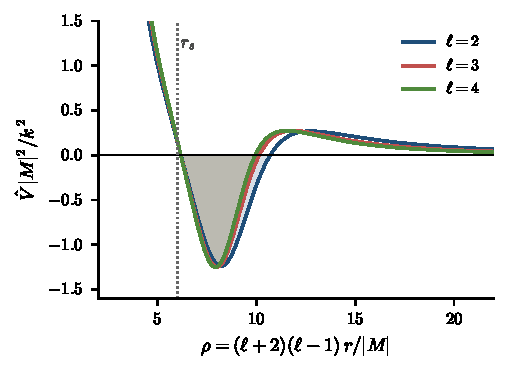
\includegraphics[width=0.48\textwidth]{fig1_vhat.pdf}
\caption{The regularised potential $\Vhat$ for $\ell=2,3,4$, in the scaled radius $\rho=cr/|M|$. Shaded: $\Vhat<0$,
which occurs only on a shell just beyond $r_s$ ($\rho=6$). With radius scaled by $c=(\ell+2)(\ell-1)$ and the
potential by the eigenvalue scale $k^2$, the curves nearly coincide.}
\label{fig:vhat}
\end{figure}

\begin{lemma}[properties of $\chi$, $\phi_0$, $\Vhat$; all $\ell\ge2$]\label{lem:props}\leavevmode
\begin{enumerate}
\item $\chi=\sum_{n=1}^{\ell+2}c_n r^n$ with $c_1=\tfrac32$, $c_2=0$, $c_3=-K/32$, $c_4=K/96$ ($K=6k$), $c_n\ge0$ for
$n\ge4$ and $c_{\ell+2}>0$; $\psi_0$ solves the static Zerilli equation identically in $\ell$; and $\chi>0$ on $r>0$.
\item At $r_s$ the $\chi$-equation has Frobenius exponents $0$ and $3$, forcing $\chi''(r_s)=0$; hence $\Vhat$ is
real-analytic on $(0,\infty)$.
\item $r^4\Vhat=12+O(r)$ as $r\to0$ (exponents $x^{3/2}$, $x^{-1/2}$), and $\Vhat\simeq(\ell+1)(\ell+2)/r^2$ as
$r\to\infty$. $\Hhat$ is limit point at both ends, hence essentially self-adjoint on $C_c^\infty(0,\infty)$.
\item $\phi_0$ is the non-admissible branch $\propto x^{-1/2}$ at $0$, decays as $r^{-(\ell+1)}$ at infinity, and has
exactly one zero, at $r_s$, which is simple.
\end{enumerate}
\end{lemma}
\begin{proof}[Sketch]
(1) The closed form $c_n=(n-2)\bigl((n-4)\ell(\ell+1)+n-1\bigr)(\ell-n+3)_{2n-4}/\bigl(2^n(n-1)!^2\bigr)$ turns the static
equation into a three-term recurrence, which becomes a polynomial identity in $(\ell,n)$ after dividing by a Pochhammer
factor; it is verified symbolically. Positivity follows Ref.~\cite{DG2009}, Eqs.~(57)--(59): dropping the non-negative
terms $n\ge6$ leaves a quartic whose unique positive critical value is
$4(K-18)(Ks-18(K-16))/[(\ell-2)(\ell+3)(\ell^2+\ell+4)]^3$, $s=\sqrt{6(K-18)}$, which is positive because
$(Ks)^2-(18(K-16))^2=6(K-24)^3>0$ for $\ell\ge3$; $\ell=2$ is checked directly. (2)--(4) are local expansions, verified
symbolically in $\ell$; limit point at $0$ holds because $x^{-1/2}\notin L^2$, and the Weyl alternative gives essential
self-adjointness~\cite{ReedSimon2,Weidmann1987}.
\end{proof}

\section{Exactly one unstable mode}\label{sec:one}

The key tool is the ground-state identity: if $\Vhat=\phi_0''/\phi_0$ and $u=\phi_0 h$, then
\begin{equation}\label{eq:gs}
u'^2+\Vhat u^2=\phi_0^2h'^2+\bigl(\phi_0\phi_0'h^2\bigr)'.
\end{equation}

\begin{theorem}\label{thm:one}
For every $\ell\ge2$, $\Hhat$ has exactly one negative eigenvalue. It is simple and equals $-(k/2)^2$, so the unique
unstable even-parity mode of negative-mass Schwarzschild grows at the Gleiser--Dotti rate $\gamma=k/(2|M|)$. Zero is
not an eigenvalue.
\end{theorem}

\begin{proof}
\emph{At most one.} By Glazman's lemma~\cite{BirmanSolomyak}, the number of negative eigenvalues equals the largest
dimension of a subspace of a form core on which $q[u]=\langle u,\Hhat u\rangle$ is negative definite. Take the core
$C_c^\infty(0,\infty)$ and suppose such a subspace $F$ has $\dim F\ge2$. Choose $u\in F\setminus\{0\}$ with $u(x_s)=0$,
$x_s=x(r_s)$. Since $\phi_0$ is analytic with a simple zero at $x_s$, $h=u/\phi_0$ is smooth, and integrating
\eqref{eq:gs} over the compact support of $u$ gives $q[u]=\int\phi_0^2h'^2\,\dd x\ge0$, a contradiction.

\emph{At least one.} The function $\hat\Psi=A^*\Psi_{\rm DG}$, with
$\Psi_{\rm DG}=r(r+2)^ke^{-kr/2}/(cr-6)$, satisfies $\Hhat\hat\Psi=-(k/2)^2\hat\Psi$ identically in $\ell$, is
$O(r^3)$ at $0$, regular at $r_s$, and decays exponentially; so it is an eigenfunction. Independently of this explicit
mode, $w=\phi_0\mathbf 1_{x>x_s}$ lies in the form domain with $q[w]=0$ by \eqref{eq:gs}; if $\Hhat\ge0$, $w$ would be a
minimiser and hence a weak, therefore $C^1$, solution of $\Hhat w=0$, contradicting the kink at $x_s$.

\emph{No zero mode.} The zero-energy solution admissible at $x=0$ is
\[
v=\phi_0F,\qquad F(r)=\mathrm{f.p.}\!\int_0^r\psi_0^2\,\frac{\dd x}{\dd r}\,\dd r ;
\]
it grows as $r^{\ell+2}$ and is not in $L^2$.
\end{proof}

\begin{remark}
$v$ has exactly one zero for every $\ell$ ($F$ is positive on $(0,r_s)$ and increases from $-\infty$ to $+\infty$ on
$(r_s,\infty)$), as renormalised oscillation theory~\cite{GST1996} requires. The proof does not use oscillation theory at
the continuum edge. Numerically, Chebyshev discretisations with $\hat\Psi=r^3u$ reproduce $E_0=-(k/2)^2$ to
$\le3\times10^{-13}$ for $\ell\le8$ and find no second bound state in 140 resolution and domain variations.
\end{remark}

\section{Finite stars: an exact count}\label{sec:trunc}

Model the exterior of a star of areal radius $R$ by $\Hhat_{R,\kappa}$ on $L^2(x_R,\infty)$ with the Robin condition
$\hat\Psi'(x_R)=\kappa\hat\Psi(x_R)$; $\kappa=+\infty$ denotes Dirichlet. The interior matter determines $\kappa$, which in
general depends on frequency and $\ell$; here it is a free parameter. Define
\begin{equation}\label{eq:kc}
\kappa_c(R)=\frac{\dd\ln\phi_0}{\dd x}\Big|_R=\Bigl(1+\frac2R\Bigr)\frac{\mathcal N(R)}{(cR-6)\chi(R)},
\qquad \mathcal N=c\chi-(cr-6)\chi'.
\end{equation}

\begin{theorem}\label{thm:trunc}
For every $\ell\ge2$ and $R\neq r_s$, the number of negative eigenvalues of $\Hhat_{R,\kappa}$ is
\begin{equation}
\Ind{R<r_s}+\Ind{\kappa<\kappa_c(R)},
\end{equation}
with Dirichlet counted as $\kappa=+\infty$. At $\kappa=\kappa_c$, $\phi_0$ is a zero-energy eigenfunction.
\end{theorem}

\begin{proof}
For $u$ in the core, \eqref{eq:gs} gives $q[u]=\int\phi_0^2h'^2\,\dd x+(\kappa-\kappa_c)u(x_R)^2$ provided $u(x_s)=0$ when
$R<r_s$. Imposing $u(x_s)=0$ (if $R<r_s$) and $u(x_R)=0$ (if $\kappa<\kappa_c$) costs at most
$\Ind{R<r_s}+\Ind{\kappa<\kappa_c}$ linear conditions and leaves $q\ge0$; Glazman's lemma gives the upper bound. For the
lower bound use $w_1=\phi_0\mathbf 1_{[x_R,x_s]}$ and $w_2=\phi_0\mathbf 1_{[x_s,\infty)}$ (or $\phi_0$ itself if
$R>r_s$), for which $q[aw_1+bw_2]=a^2\phi_0(x_R)^2(\kappa-\kappa_c)$ and $q[w_2]=0$. If the negative spectral subspace
were smaller, some combination orthogonal to it would have $q=0$, hence be a weak zero-energy solution satisfying the
boundary condition; the kink of $w_2$, or $\kappa\ne\kappa_c$, excludes this.
\end{proof}

\begin{corollary}[thresholds, all $\ell$]\label{cor:thr}
$\mathcal N>0$ on $[0,r_s]$ and has exactly one root $r_*>r_s$. Hence $\kappa_c<0$ on $(0,r_s)$, $\kappa_c\to\mp\infty$
at $r_s^\mp$, $\kappa_c>0$ on $(r_s,r_*)$ and $\kappa_c<0$ on $(r_*,\infty)$. In particular:
Dirichlet is unstable iff $R<r_s$; Neumann is unstable iff $R<r_*$; every $\kappa\ge0$ is stable iff $R\ge r_*$.
\end{corollary}

The first claim follows from a telescoping lower bound on $[0,r_s]$; uniqueness of $r_*$ from Descartes' rule applied to
$\mathcal N(r_s+t)$, whose coefficients have one sign change because $\chi''(r_s)=0$ and $\chi^{(m)}(r_s)>0$ for
$m\ge4$. Table~\ref{tab:thr} lists the thresholds and Fig.~\ref{fig:kc} the critical surface condition. Asymptotically,
\begin{align}
\kappa_c&=-\frac{\ell+1}{R}-\frac{\ell^4+3\ell^3+4\ell^2+4}{\ell(\ell-1)(\ell+2)}\frac{1}{R^2}+O(R^{-3})
&&(R\to\infty),\\
\kappa_c\,x_R&=-\frac12-\frac{(\ell^2+\ell-1)R}{12}+O(R^2)&&(R\to0).
\end{align}
For large $R$ an instability therefore requires a surface condition softer than the static vacuum tail
$\phi_0\propto r^{-(\ell+1)}$ by an $O(1)$ factor on the scale $1/R$. As $R\to0$ every condition with
$\kappa x_R>-\tfrac12$ (including Dirichlet and Neumann) reproduces the Dotti--Gleiser eigenvalue, with error scaling
roughly as $R^3$--$R^4$, so the self-adjoint extension of Ref.~\cite{DG2009} is the limit of a regular cutoff; compare
the scalar-wave analysis of Ref.~\cite{Giveon2004}.

\begin{table}[t]
\centering
\begin{tabular}{cccccc}
\toprule
$\ell$ & $r_s$ & $r_*$ & $r_{\rm neg}$ & $\gamma_{\rm DG}=k/2$ & $|M|/r_*$\\
\midrule
2 & 1.5000 & 2.2788 & 2.6741 & 2 & 0.439\\
3 & 0.6000 & 0.8789 & 1.0143 & 10 & 1.14\\
4 & 0.3333 & 0.4814 & 0.5519 & 30 & 2.08\\
5 & 0.2143 & 0.3073 & 0.3512 & 70 & 3.25\\
\bottomrule
\end{tabular}
\caption{Thresholds in units of $|M|$. $r_s$: Dirichlet threshold; $r_*$: Neumann and $\kappa\ge0$ threshold;
$r_{\rm neg}=\sup\{r:\Vhat<0\}$. Since $r_*$ decreases with $\ell$ (checked for $\ell\le80$), a star with
$|M|/R<0.439$ and $\kappa\ge0$ has no unstable even-parity mode for any $\ell$. At large
$\ell$, $r_*\approx8.486/c$ and $r_{\rm neg}\approx9.636/c$ (derived from the $\ell\to\infty$ limit of $c\,\chi(\rho/c)$, a
modified-Bessel closed form; convergence of the roots is not proven).}
\label{tab:thr}
\end{table}

\begin{figure}[t]
\centering
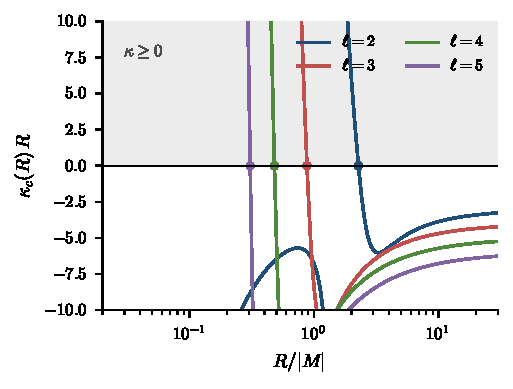
\includegraphics[width=0.48\textwidth]{fig2_kappa_c.pdf}\hfill
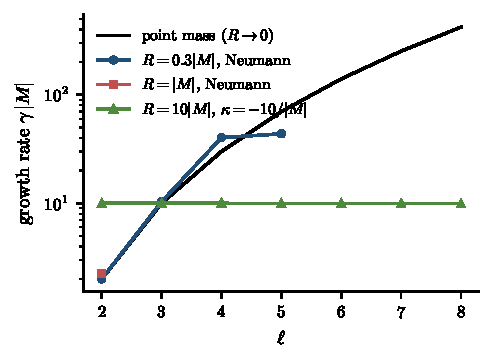
\includegraphics[width=0.48\textwidth]{fig3_growth.pdf}
\caption{Left: critical surface condition $\kappa_c(R)R$ for $\ell=2$--$5$. A mode is unstable when $\kappa<\kappa_c$,
plus one unconditional mode when $R<r_s$ (pole). Dots mark $r_*$. Above $r_*$ the whole $\kappa\ge0$ region (shaded) is
stable. Right: growth rate versus $\ell$. The point mass grows as $\ell^4/12$; any finite $R$ with an $\ell$-independent
condition leaves finitely many unstable $\ell$ ($\kappa\ge0$) or caps the rate at $|\kappa|$ ($\kappa<0$, since
$\Vhat\ge0$ outside $r_{\rm neg}$).}
\label{fig:kc}
\end{figure}

\paragraph{Growth-rate cap.} For the point mass the growth rate $k/2\sim\ell^4/12$ is unbounded in $\ell$. For a star:
with $\kappa\ge0$ only $\ell$ with $R<r_*(\ell)$, roughly $\ell\lesssim3/\sqrt{R}$, are unstable; with a fixed $\kappa<0$,
every $\ell$ with $r_{\rm neg}(\ell)<R$ has $\Vhat\ge0$ outside the star and growth $\le|\kappa|$. Either way
$\sup_\ell\gamma<\infty$ (Fig.~\ref{fig:kc}, right; a 1000-case numerical scan agrees with Theorem~\ref{thm:trunc}).
The unbounded growth belongs to the singularity.

\section{Discussion}\label{sec:discussion}

For the point mass, Theorem~\ref{thm:one} completes the linear stability analysis: negative-mass Schwarzschild has
one unstable even-parity mode per $\ell$, at the Gleiser--Dotti rate, and no others. Theorem~\ref{thm:trunc} shows where that
mode lives. The negative part of the effective potential sits on a shell of radius $\approx10|M|/\ell^2$
(Fig.~\ref{fig:vhat}); a star whose surface lies outside $r_*(\ell)$ hides it unless its interior supplies an
energy-injecting surface condition, and for $\ell=2$ the condition is $|M|/R<0.439$. In this sense the instability is a
point-mass effect, contrary to the suggestion in Ref.~\cite{Dotti2022}: for a dilute regular source the vacuum exterior
cannot drive it, and the $\ell^4$ growth disappears.

Which side of $\kappa_c$ a real star lies on is a property of its matter. For the phantom boson star of
Ref.~\cite{Shirokov2026} the companion paper~\cite{Moinvaziri2026b} finds $\kappa_{\rm eff}>\kappa_c$ for $\ell=2$, together
with the identity $\kappa_{\rm eff}-\kappa_c=s^2/(q_{\rm int}-g)$, so the threshold of Theorem~\ref{thm:trunc} is the
natural yardstick for any regular source. A limitation: the Robin model is exact only for an interface condition
independent of frequency; a real star supplies a frequency-dependent one, for which Theorem~\ref{thm:trunc} gives the
count at each fixed frequency.

\section{How the results were obtained}\label{sec:method}

The author set the questions and scope and reviewed each stage; Anthropic's Claude, run as an agent with a Python
environment and parallel sub-agents, did the literature reading, derivations, code and drafting. No claim rests on
the assistant's word alone:
\begin{itemize}
\item \emph{Starting points.} Published results were re-derived before use, exposing a sign misprint in
Ref.~\cite{DG2009} and the discontinuous mode of Ref.~\cite{GHI2005}.
\item \emph{Proofs.} Every identity behind Lemma~\ref{lem:props} and Theorems~\ref{thm:one}--\ref{thm:trunc} was verified
in exact arithmetic (SymPy), and the predicted mode counts were confirmed by a 1000-case spectral scan.
\item \emph{Review.} A literature search preceded every novelty claim; the zero mode $\phi_0$ is credited to
Ref.~\cite{DG2009}.
\end{itemize}
These checks are internal; the work has not yet been reviewed by specialists.

\paragraph{Reproducibility.} The symbolic verifications (exact for $\ell=2$--$10$ and symbolically in $\ell$ where
stated; root isolation of $\mathcal N$ for $\ell\le50$), the spectral computations and the figure script are in the
accompanying repository.

\paragraph{Acknowledgments.} The author thanks Anthropic's Claude, which carried out the analysis, computations and
drafting described in Sec.~\ref{sec:method} under the author's direction.

\begin{thebibliography}{99}

\bibitem{Bondi1957} H. Bondi, ``Negative mass in general relativity,'' Rev. Mod. Phys. \textbf{29}, 423 (1957).
\bibitem{Shirokov2026} N. M. Shirokov, ``The Bondi dipole in full numerical relativity: a self-accelerating
positive--negative mass binary,'' arXiv:2608.24577.
\bibitem{GHI2005} G. W. Gibbons, S. A. Hartnoll and A. Ishibashi, ``On the stability of naked singularities,''
Prog. Theor. Phys. \textbf{113}, 963 (2005), arXiv:hep-th/0409307.
\bibitem{GD2006} R. J. Gleiser and G. Dotti, ``Instability of the negative mass Schwarzschild naked singularity,''
Class. Quantum Grav. \textbf{23}, 5063 (2006), arXiv:gr-qc/0604021.
\bibitem{DG2009} G. Dotti and R. J. Gleiser, ``The initial value problem for linearized gravitational perturbations of
the Schwarzschild naked singularity,'' Class. Quantum Grav. \textbf{26}, 215002 (2009), arXiv:0809.3615.
\bibitem{CC2006} V. Cardoso and M. Cavagli\`a, ``Stability of naked singularities and algebraically special modes,''
Phys. Rev. D \textbf{74}, 024027 (2006), arXiv:gr-qc/0604101.
\bibitem{Dotti2022} G. Dotti, ``Linear stability of black holes and naked singularities,'' Universe \textbf{8}, 38
(2022), arXiv:2201.03640.
\bibitem{MP2014} S. Mbarek and M. B. Paranjape, ``Negative mass bubbles in de Sitter space-time,'' Phys. Rev. D
\textbf{90}, 101502 (2014), arXiv:1407.1457.
\bibitem{Johnson2020} M. C. Johnson, M. B. Paranjape, A. Savard and A. Tapia-Arellano, ``Stable, thin wall, negative mass
bubbles in de Sitter space-time,'' arXiv:1910.01774.
\bibitem{Alves2025} M. de Aguiar Alves, A. G. S. Landulfo and B. Arderucio Costa, arXiv:2408.00154; Phys. Rev. D
\textbf{111}, 044027 (2025).
\bibitem{Moinvaziri2026b} N. Moinvaziri, ``Stability of a negative-mass boson star,'' companion paper (2026).
\bibitem{Zerilli1970} F. J. Zerilli, ``Effective potential for even-parity Regge--Wheeler gravitational perturbation
equations,'' Phys. Rev. Lett. \textbf{24}, 737 (1970); Phys. Rev. D \textbf{2}, 2141 (1970).
\bibitem{ReedSimon2} M. Reed and B. Simon, \emph{Methods of Modern Mathematical Physics II: Fourier Analysis,
Self-Adjointness} (Academic Press, 1975).
\bibitem{Weidmann1987} J. Weidmann, \emph{Spectral Theory of Ordinary Differential Operators}, Lecture Notes in
Mathematics 1258 (Springer, 1987).
\bibitem{BirmanSolomyak} M. Sh. Birman and M. Z. Solomyak, \emph{Spectral Theory of Self-Adjoint Operators in Hilbert
Space} (Reidel, 1987).
\bibitem{GST1996} F. Gesztesy, B. Simon and G. Teschl, ``Zeros of the Wronskian and renormalized oscillation theory,''
Amer. J. Math. \textbf{118}, 571 (1996).
\bibitem{Giveon2004} A. Giveon, B. Kol, A. Ori and A. Sever, ``On the resolution of the time-like singularities in
Reissner--Nordstr\"om and negative-mass Schwarzschild,'' JHEP \textbf{08}, 014 (2004), arXiv:hep-th/0401209.

\end{thebibliography}

\end{document}
